\documentclass[11pt]{article}

% ---------- Packages (per course conventions) ----------
\usepackage[margin=1in]{geometry}
\usepackage{graphicx}
\usepackage{float}
\usepackage{booktabs}
\usepackage{siunitx}
\usepackage{amsmath}
\usepackage{amssymb}
\usepackage{tikz}
\usetikzlibrary{arrows.meta,calc,patterns,decorations.pathmorphing}
\usepackage{tcolorbox}
\usepackage{enumitem}
\usepackage{xcolor}
\usepackage{hyperref}
\hypersetup{colorlinks=true, linkcolor=black, urlcolor=blue}

\setlength{\parindent}{0pt}
\setlength{\parskip}{0.6\baselineskip}

\sisetup{per-mode=symbol}
\DeclareSIUnit{\lb}{lb}
\DeclareSIUnit{\ft}{ft}
\DeclareSIUnit{\inch}{in}
\DeclareSIUnit{\kip}{kip}

% =========================================================
\newcommand{\assignmentNumber}{8}
\newcommand{\assignedDate}{8 Nov 2024}
\newcommand{\dueDate}{15 Nov 2024 (11:59pm on Moodle)}

% ---------- Boxed-answer helper ----------
\newtcolorbox{finalanswer}{
    colback=white, colframe=black, boxrule=1pt,
    title=Answer, fonttitle=\bfseries, coltitle=black,
    colbacktitle=white
}

% ---------- Problem header (each problem starts on a new page) ----------
\newcommand{\problem}[1]{\clearpage\section*{Problem #1}}

% ---------- TikZ styles ----------
\tikzset{
    body/.style={draw=black, fill=blue!10!gray!22, thick},
    load/.style={-{Stealth[length=2.8mm]}, very thick, red!75!black},
    react/.style={-{Stealth[length=2.8mm]}, very thick, blue!70!black},
    dim/.style={{Latex[length=1.6mm]}-{Latex[length=1.6mm]}, thin},
    ext/.style={thin, gray},
    motion/.style={-{Stealth[length=2.2mm]}, dashed, thick, gray!60!black},
    lbl/.style={font=\small},
}
% axes: \axes{(x,y)}
\newcommand{\axes}[1]{%
    \begin{scope}[shift={#1}]
        \draw[-{Stealth},thin] (0,0)--(0.7,0) node[right]{\footnotesize $x$};
        \draw[-{Stealth},thin] (0,0)--(0,0.7) node[above]{\footnotesize $y$};
    \end{scope}}
\newcommand{\legendline}{\par\footnotesize\textcolor{red!75!black}{\textbf{Red}}: applied loads and weights.\quad
    \textcolor{blue!70!black}{\textbf{Blue}}: reactions (normal and friction).\quad
    \textcolor{gray!60!black}{\textbf{Dashed gray}}: direction of impending motion.\normalsize\par}

\begin{document}

% =========================================================
% COVERSHEET
% =========================================================
\begin{titlepage}
    \centering
    \vspace*{2cm}
    {\LARGE \bfseries ENGR 225: Mechanics 1} \\[0.3cm]
    {\Large Homework Coversheet} \\[0.3cm]
    {\large Assoc.\ Prof.\ Clayton Byers} \\[2cm]

    \begin{flushleft}
        \Large
        \textbf{NAME:} \underline{\makebox[10cm][l]{\ Sean Balbale}} \\[1cm]
        \textbf{DATE:} \underline{\makebox[10cm][l]{\ }} \\[1cm]
        \textbf{ASSIGNMENT:} \underline{\makebox[9cm][l]{\ Homework 8}} \\[2cm]
    \end{flushleft}

    \large
    \textbf{Level of involvement of AI, LLMs, or related tools in the completion of this assignment:}

    \vspace{1cm}

    \begin{flushleft}
        \Large
        $\square$ \quad None \\[0.7cm]
        $\square$ \quad Minor \\[0.7cm]
        $\square$ \quad Major \\[0.7cm]
        $\square$ \quad Extensive \\[1.5cm]
    \end{flushleft}

    \normalsize
    \textit{Mark the box that applies (e.g., replace $\square$ with $\blacksquare$, or type an X beside it, before compiling/printing). Your disclosure does not affect your grade -- it keeps you accountable for the work you are doing.}
\end{titlepage}

% =========================================================
% HOMEWORK HEADER
% =========================================================
\section*{ENGR 225 -- Homework \assignmentNumber}
\textbf{Assigned:} \assignedDate \hfill \textbf{Due:} \dueDate

\textit{Each problem starts on its own page, with a problem summary, labeled sketch, governing equations, units carried throughout, results to 3 significant figures, and a boxed final answer.}

\textbf{Conventions used throughout.} Moments are positive counterclockwise. Every friction problem is set up at \emph{impending} motion, so wherever slip is assumed the friction force equals $\mu_s N$ and points opposite the direction the surface would slide. Free-body diagram colors:
\legendline

% =========================================================
% PROBLEM 1
% =========================================================
\problem{1}

\textbf{Given / Find:} A wheel of radius \SI{150}{mm} carries a \SI{5}{N.m} clockwise torque. A lever pinned at $A$ presses friction block $B$ against the bottom of the wheel ($\mu_s = 0.3$). The contact at $B$ sits \SI{200}{mm} right of and \SI{50}{mm} below the pin, and $P$ acts upward \SI{400}{mm} further right. Determine whether the brake holds the wheel for $P = \SI{30}{N}$ and $P = \SI{70}{N}$.

\textbf{Sketch:}

\begin{center}
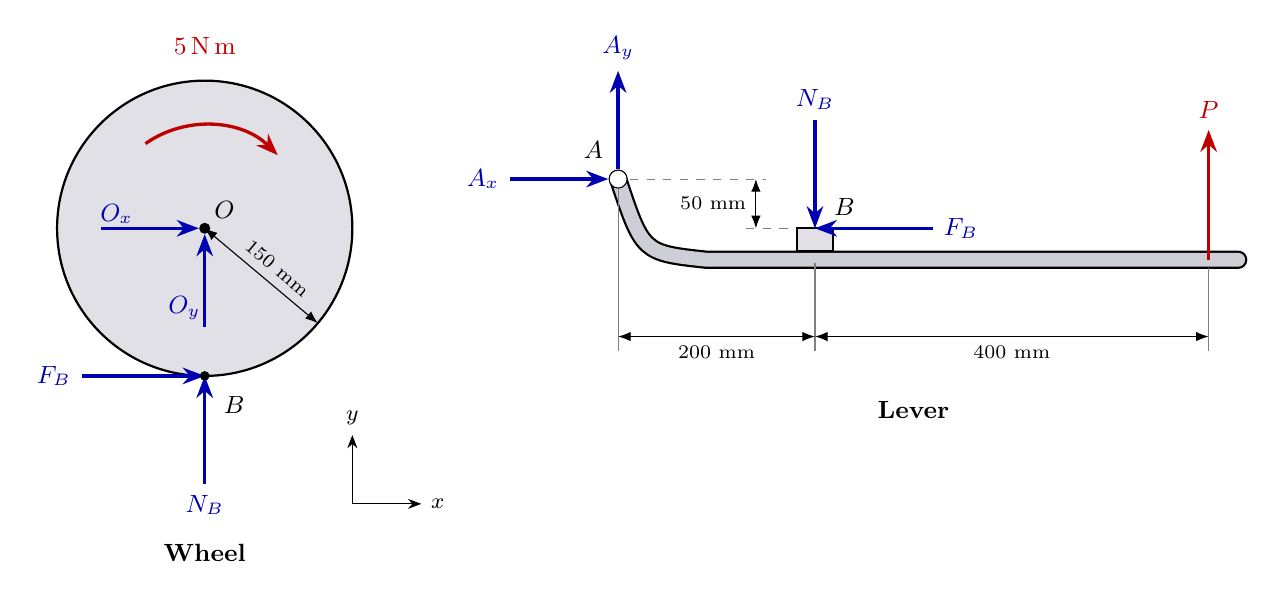
\begin{tikzpicture}[scale=1.25]
    % ---------- Wheel FBD ----------
    \begin{scope}
        \draw[body] (0,0) circle (1.5);
        \fill (0,0) circle (1.6pt) node[above right, lbl]{$O$};
        \draw[dim] (0,0) -- (320:1.5) node[pos=0.55, above, sloped, font=\scriptsize]{150 mm};
        \draw[load] (125:1.05) arc[start angle=125, end angle=45, radius=1.05];
        \node[lbl, red!75!black] at (0,1.85) {\SI{5}{N.m}};
        \draw[react] (-1.05,0.0) -- (-0.06,0.0) node[pos=0, above right, lbl, fill=blue!10!gray!22, inner sep=1pt, xshift=-2pt]{$O_x$};
        \draw[react] (0,-1.0) -- (0,-0.06) node[pos=0.2, left, lbl, fill=blue!10!gray!22, inner sep=1pt]{$O_y$};
        \draw[react] (0,-2.6) -- (0,-1.5) node[pos=0, below, lbl]{$N_B$};
        \draw[react] (-1.25,-1.5) -- (0,-1.5) node[pos=0, left, lbl]{$F_B$};
        \fill (0,-1.5) circle (1.4pt);
        \node[lbl] at (0.3,-1.8) {$B$};
        \node[font=\bfseries\small] at (0,-3.3) {Wheel};
        \axes{(1.5,-2.8)}
    \end{scope}

    % ---------- Lever FBD ----------
    \begin{scope}[shift={(4.2,0.5)}]
        % lever (tube)
        \draw[double=blue!10!gray!35, double distance=5pt, thick, line cap=round]
            (0,0) .. controls (0.25,-0.75) .. (0.9,-0.82) -- (6.3,-0.82);
        % friction block
        \draw[body] (1.82,-0.73) rectangle (2.18,-0.5);
        \fill[white] (0,0) circle (2.6pt); \draw (0,0) circle (2.6pt);
        \node[lbl] at (-0.25,0.3) {$A$};
        % pin reactions
        \draw[react] (-1.1,0) -- (-0.1,0) node[pos=0, left, lbl]{$A_x$};
        \draw[react] (0,0.1) -- (0,1.1) node[above, lbl]{$A_y$};
        % contact forces on lever
        \draw[react] (2,0.6) -- (2,-0.5) node[pos=0, above, lbl]{$N_B$};
        \draw[react] (3.2,-0.5) -- (2,-0.5) node[pos=0, right, lbl]{$F_B$};
        \node[lbl] at (2.3,-0.28) {$B$};
        % applied load
        \draw[load] (6,-0.82) -- (6,0.5) node[above, lbl]{$P$};
        % dimensions
        \draw[ext] (0,-0.1) -- (0,-1.75);
        \draw[ext] (2,-0.85) -- (2,-1.75);
        \draw[ext] (6,-0.9) -- (6,-1.75);
        \draw[dim] (0,-1.6) -- (2,-1.6) node[midway, below, font=\scriptsize]{200 mm};
        \draw[dim] (2,-1.6) -- (6,-1.6) node[midway, below, font=\scriptsize]{400 mm};
        \draw[ext, dashed] (0.12,0) -- (1.5,0);
        \draw[ext, dashed] (1.3,-0.5) -- (1.8,-0.5);
        \draw[dim] (1.4,0) -- (1.4,-0.5) node[midway, left, font=\scriptsize]{50 mm};
        \node[font=\bfseries\small] at (3,-2.35) {Lever};
    \end{scope}
\end{tikzpicture}
\end{center}

The clockwise torque would turn the bottom of the wheel to the left, so friction on the wheel at $B$ points right. By Newton's third law, friction on the lever points left and $N_B$ pushes the lever down.

\textbf{Solution:}

\textit{Wheel.} The friction force required to hold the wheel does not depend on $P$:
\begin{align*}
    \sum M_O &= F_B(\SI{0.150}{m}) - \SI{5}{N.m} = 0 \quad\Rightarrow\quad F_B = \SI{33.3}{N}
\end{align*}

\textit{Lever.} Moments about $A$ eliminate the pin reactions. $F_B$ acts \SI{50}{mm} below $A$, so it contributes a moment:
\begin{align*}
    \sum M_A &= P(\SI{0.600}{m}) - N_B(\SI{0.200}{m}) - F_B(\SI{0.050}{m}) = 0 \\
    \Rightarrow\quad N_B &= \frac{P(\SI{0.600}{m}) - (\SI{33.3}{N})(\SI{0.050}{m})}{\SI{0.200}{m}}
\end{align*}

\textit{Slip check.} The brake holds only if the required friction does not exceed the maximum available, $F_B \le (F_B)_{\max} = \mu_s N_B$.

\begin{center}
\begin{tabular}{cccl}
    \toprule
    $P$ & $N_B$ & $(F_B)_{\max} = 0.3N_B$ & vs.\ \SI{33.3}{N} required \\
    \midrule
    \SI{30}{N} & \SI{81.7}{N} & \SI{24.5}{N} & $24.5 < 33.3 \;\Rightarrow\;$ slips \\
    \SI{70}{N} & \SI{202}{N} & \SI{60.5}{N} & $60.5 > 33.3 \;\Rightarrow\;$ holds \\
    \bottomrule
\end{tabular}
\end{center}

\begin{finalanswer}
    $P = \SI{30}{N}$: $(F_B)_{\max} = \SI{24.5}{N} < \SI{33.3}{N}$, so the brake \textbf{cannot} hold the wheel. \\
    $P = \SI{70}{N}$: $(F_B)_{\max} = \SI{60.5}{N} > \SI{33.3}{N}$, so the brake \textbf{can} hold the wheel.
\end{finalanswer}

% =========================================================
% PROBLEM 2
% =========================================================
\problem{2}

\textbf{Given / Find:} A uniform \SI{30}{\lb}, \SI{26}{\ft} pole leans against a smooth wall at $B$ and rests on a rough floor at $A$ ($\mu_s = 0.3$), with $A$ a distance $d = \SI{10}{\ft}$ from the wall. Determine whether the pole stays in place when released.

\textbf{Sketch:}

\begin{center}
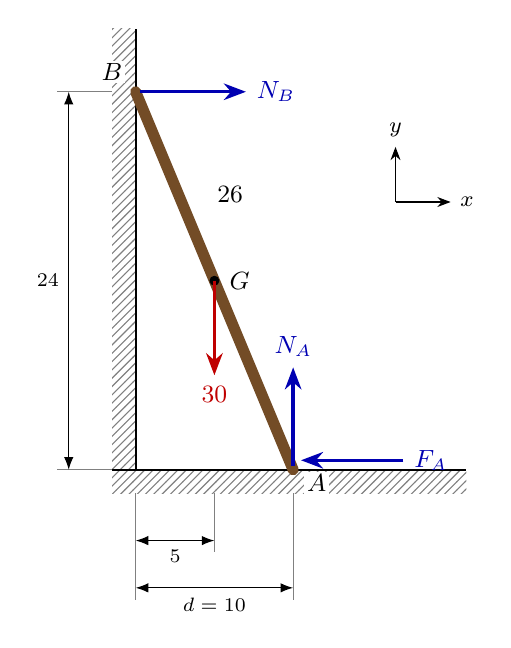
\begin{tikzpicture}[scale=1.0]
    % wall and floor (for reference)
    \fill[pattern=north east lines, pattern color=gray] (-0.3,0) rectangle (0,5.6);
    \draw[thick] (0,0) -- (0,5.6);
    \fill[pattern=north east lines, pattern color=gray] (-0.3,-0.3) rectangle (4.2,0);
    \draw[thick] (-0.3,0) -- (4.2,0);
    % pole
    \draw[line width=4pt, brown!60!black, line cap=round] (2,0) -- (0,4.8);
    \fill (1,2.4) circle (1.8pt) node[right, lbl, xshift=2pt]{$G$};
    \node[lbl, fill=white, inner sep=1pt] at (-0.3,5.05) {$B$};
    \node[lbl, fill=white, inner sep=1pt] at (2.3,-0.17) {$A$};
    \node[lbl] at (1.2,3.5) {\SI{26}{\ft}};
    % forces
    \draw[load] (1,2.4) -- (1,1.2) node[below, lbl]{\SI{30}{\lb}};
    \draw[react] (0.05,4.8) -- (1.4,4.8) node[right, lbl]{$N_B$};
    \draw[react] (2,0.05) -- (2,1.3) node[above, lbl]{$N_A$};
    \draw[react] (3.4,0.12) -- (2.1,0.12) node[pos=0, right, lbl]{$F_A$};
    % dimensions
    \draw[ext] (2,-0.3) -- (2,-1.65);
    \draw[ext] (1,-0.3) -- (1,-1.05);
    \draw[ext] (0,-0.3) -- (0,-1.65);
    \draw[dim] (0,-0.9) -- (1,-0.9) node[midway, below, font=\scriptsize]{\SI{5}{\ft}};
    \draw[dim] (0,-1.5) -- (2,-1.5) node[midway, below, font=\scriptsize]{$d = \SI{10}{\ft}$};
    \draw[ext] (-0.3,4.8) -- (-1.0,4.8);
    \draw[ext] (-0.3,0) -- (-1.0,0);
    \draw[dim] (-0.85,0) -- (-0.85,4.8) node[midway, left, font=\scriptsize]{\SI{24}{\ft}};
    \axes{(3.3,3.4)}
\end{tikzpicture}
\end{center}

The smooth wall can only push horizontally, so $N_B$ is the only force at $B$. If the pole slid, $A$ would move away from the wall, so friction at $A$ points toward the wall.

\textbf{Solution:}

\textit{Geometry.} Height of $B$ above the floor:
\[
    h = \sqrt{(\SI{26}{\ft})^2 - (\SI{10}{\ft})^2} = \SI{24}{\ft}
\]
The weight acts at the midpoint $G$, \SI{5}{\ft} from the wall and \SI{5}{\ft} horizontally from $A$.

\textit{Equilibrium.} Assume the pole stays put and solve for the friction it needs:
\begin{align*}
    \sum F_y &= N_A - \SI{30}{\lb} = 0 &&\Rightarrow\quad N_A = \SI{30.0}{\lb} \\
    \sum M_A &= (\SI{30}{\lb})(\SI{5}{\ft}) - N_B(\SI{24}{\ft}) = 0 &&\Rightarrow\quad N_B = \SI{6.25}{\lb} \\
    \sum F_x &= N_B - F_A = 0 &&\Rightarrow\quad F_A = \SI{6.25}{\lb}
\end{align*}

\textit{Slip check.} Maximum friction available at $A$:
\[
    (F_A)_{\max} = \mu_s N_A = 0.3(\SI{30.0}{\lb}) = \SI{9.00}{\lb}
\]
Since $F_A = \SI{6.25}{\lb} < \SI{9.00}{\lb}$, the floor can supply the friction needed.

\begin{finalanswer}
    $F_A = \SI{6.25}{\lb} < (F_A)_{\max} = \SI{9.00}{\lb}$, so the pole \textbf{remains in place} when released.
\end{finalanswer}

% =========================================================
% PROBLEM 3
% =========================================================
\problem{3}

\textbf{Given / Find:} A \SI{200}{\lb} person pushes horizontally on the top right corner of a \SI{450}{\lb} crate that is \SI{2}{\ft} wide and \SI{3}{\ft} tall. The crate--floor contact has $\mu_s = 0.3$; the shoe--floor contact has $\mu_s = 0.6$. Determine whether the person can move the crate (by sliding or tipping).

\textbf{Sketch:}

\begin{center}
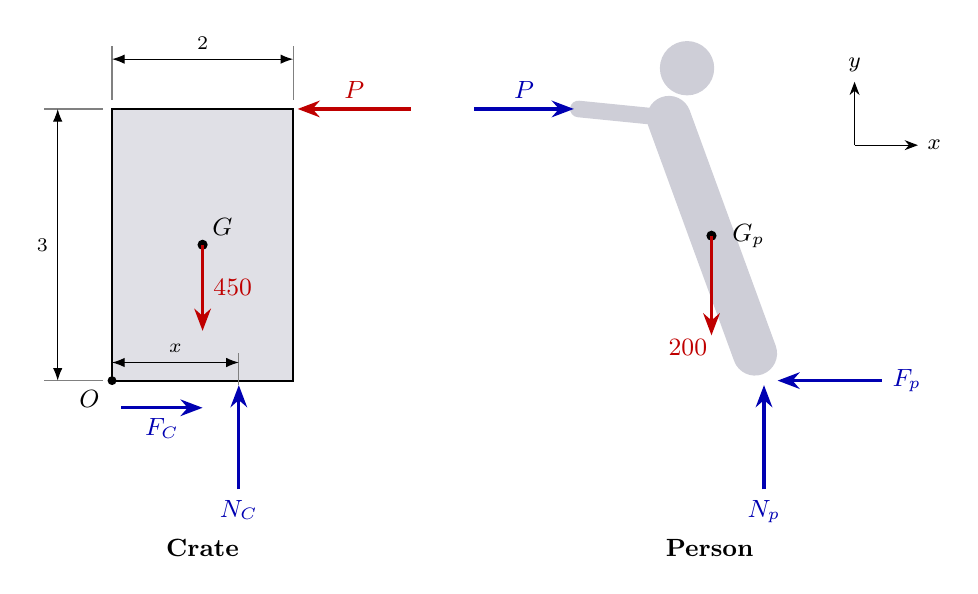
\begin{tikzpicture}[scale=1.15]
    % ---------- Crate FBD ----------
    \begin{scope}
        \draw[body] (0,0) rectangle (2,3);
        \fill (1,1.5) circle (1.6pt) node[above right, lbl]{$G$};
        \node[lbl] at (-0.25,-0.2) {$O$};
        \fill (0,0) circle (1.4pt);
        \draw[load] (3.3,3) -- (2.05,3) node[midway, above, lbl]{$P$};
        \draw[load] (1,1.5) -- (1,0.55) node[midway, right, lbl]{\SI{450}{\lb}};
        \draw[react] (1.4,-1.2) -- (1.4,-0.05) node[pos=0, below, lbl]{$N_C$};
        \draw[react] (0.1,-0.3) -- (1.0,-0.3) node[midway, below, lbl]{$F_C$};
        % dims
        \draw[ext] (0,3.1) -- (0,3.7); \draw[ext] (2,3.1) -- (2,3.7);
        \draw[dim] (0,3.55) -- (2,3.55) node[midway, above, font=\scriptsize]{\SI{2}{\ft}};
        \draw[ext] (-0.1,0) -- (-0.75,0); \draw[ext] (-0.1,3) -- (-0.75,3);
        \draw[dim] (-0.6,0) -- (-0.6,3) node[midway, left, font=\scriptsize]{\SI{3}{\ft}};
        \draw[ext] (1.4,-0.05) -- (1.4,0.3);
        \draw[dim] (0,0.2) -- (1.4,0.2) node[midway, above, font=\scriptsize]{$x$};
        \node[font=\bfseries\small] at (1,-1.85) {Crate};
    \end{scope}

    % ---------- Person FBD ----------
    \begin{scope}[shift={(5.6,0)}]
        \draw[line width=16pt, line cap=round, blue!10!gray!35] (1.5,0.3) -- (0.55,2.9);
        \draw[line width=6pt, line cap=round, blue!10!gray!35] (0.55,2.9) -- (-0.45,3);
        \fill[blue!10!gray!35] (0.75,3.45) circle (0.3);
        \fill (1.02,1.6) circle (1.6pt) node[right, lbl, xshift=4pt]{$G_p$};
        \draw[react] (-1.6,3) -- (-0.5,3) node[midway, above, lbl]{$P$};
        \draw[load] (1.02,1.6) -- (1.02,0.5) node[below left, lbl, inner sep=1pt]{\SI{200}{\lb}};
        \draw[react] (1.6,-1.2) -- (1.6,-0.05) node[pos=0, below, lbl]{$N_p$};
        \draw[react] (2.9,0) -- (1.75,0) node[pos=0, right, lbl]{$F_p$};
        \node[font=\bfseries\small] at (1,-1.85) {Person};
        \axes{(2.6,2.6)}
    \end{scope}
\end{tikzpicture}
\end{center}

$P$ pushes the crate to the left, so the crate pushes the person to the right with the same $P$, and the floor's friction on the person, $F_p$, points left. The crate either slides or tips about its bottom left corner $O$; tipping is the case where $N_C$ moves to $O$ ($x = 0$).

\textbf{Solution:}

\textit{Person (largest push they can make).} The push is horizontal, so the floor carries all of their weight:
\begin{align*}
    \sum F_y &= N_p - \SI{200}{\lb} = 0 &&\Rightarrow\quad N_p = \SI{200}{\lb} \\
    \sum F_x &= P - F_p = 0, \quad F_p \le 0.6N_p &&\Rightarrow\quad P_{\max} = 0.6(\SI{200}{\lb}) = \SI{120}{\lb}
\end{align*}

\textit{Crate, slipping.} With $F_C = \mu_s N_C$:
\begin{align*}
    \sum F_y &= N_C - \SI{450}{\lb} = 0 &&\Rightarrow\quad N_C = \SI{450}{\lb} \\
    \sum F_x &= F_C - P = 0 &&\Rightarrow\quad P_{\text{slip}} = 0.3(\SI{450}{\lb}) = \SI{135}{\lb}
\end{align*}

\textit{Crate, tipping.} With $N_C$ at $O$ ($x = 0$):
\begin{align*}
    \sum M_O &= P(\SI{3}{\ft}) - (\SI{450}{\lb})(\SI{1}{\ft}) = 0 &&\Rightarrow\quad P_{\text{tip}} = \SI{150}{\lb}
\end{align*}

The crate would slide first, at \SI{135}{\lb}. That said, the most the person can push before their own shoes slip is \SI{120}{\lb}, and $\SI{120}{\lb} < \SI{135}{\lb} < \SI{150}{\lb}$.

\begin{finalanswer}
    $P_{\max} = \SI{120}{\lb}$ (shoes slip) $< P_{\text{slip}} = \SI{135}{\lb} < P_{\text{tip}} = \SI{150}{\lb}$. \\
    The person \textbf{cannot} move the crate; it neither slides nor tips.
\end{finalanswer}

% =========================================================
% PROBLEM 4
% =========================================================
\problem{4}

\textbf{Given / Find:} Two weightless rods $AC$ and $BC$, each of length $L$, are pinned at $C$ and stand on a rough floor at $A$ and $B$ ($\mu_s = 0.6$ at both). A cylinder of unknown weight $W$ hangs from $C$, and each rod makes angle $\theta$ with the vertical. Find the largest $\theta$ for which the frame stays in equilibrium for any $W$.

\textbf{Sketch:}

\begin{center}
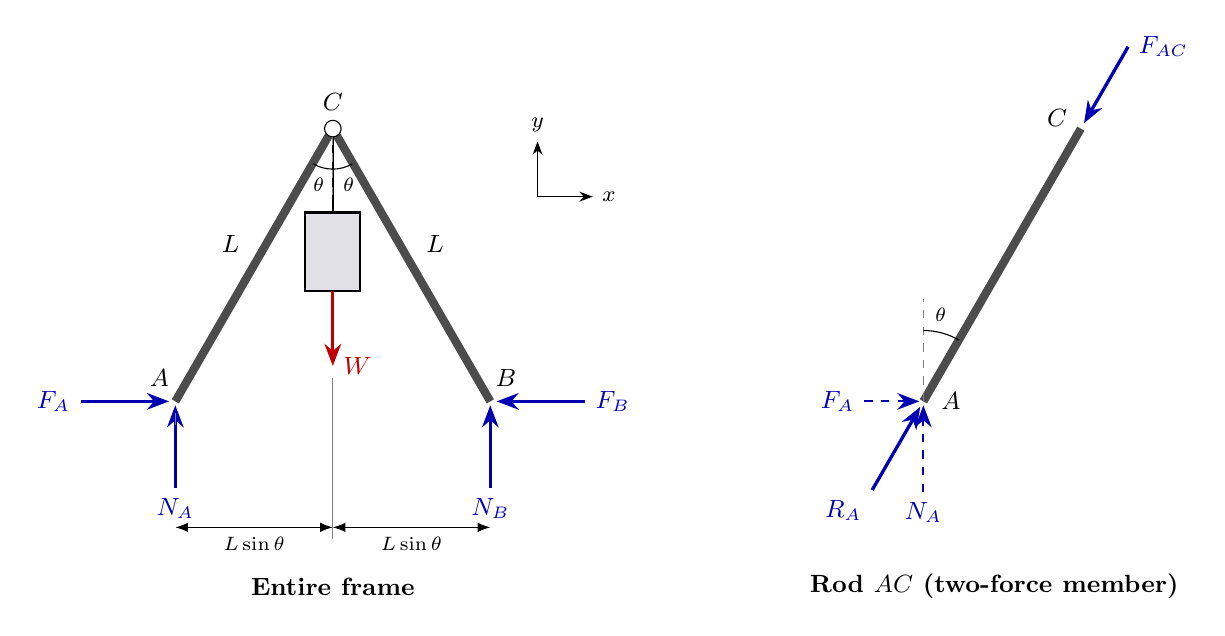
\begin{tikzpicture}[scale=1.0]
    % ---------- Whole frame ----------
    \begin{scope}
        \coordinate (A) at (-2,0); \coordinate (B) at (2,0); \coordinate (C) at (0,3.464);
        \draw[line width=3pt, gray!60!black] (A) -- (C) -- (B);
        \fill[white] (C) circle (3pt); \draw (C) circle (3pt);
        \draw[thick] (0,3.36) -- (0,2.4);
        \draw[body] (-0.35,1.4) rectangle (0.35,2.4);
        \draw[ext, dashed] (0,3.36) -- (0,2.6);
        \draw[thin] (0,2.95) arc[start angle=-90, end angle=-120, radius=0.5];
        \draw[thin] (0,2.95) arc[start angle=-90, end angle=-60, radius=0.5];
        \node[font=\scriptsize] at (-0.18,2.75) {$\theta$};
        \node[font=\scriptsize] at (0.2,2.75) {$\theta$};
        \node[lbl] at (0,3.8) {$C$};
        \node[lbl] at (-2.2,0.3) {$A$};
        \node[lbl] at (2.2,0.3) {$B$};
        \node[lbl] at (-1.3,2.0) {$L$};
        \node[lbl] at (1.3,2.0) {$L$};
        \draw[load] (0,1.4) -- (0,0.45) node[right, lbl]{$W$};
        \draw[react] (-2,-1.1) -- (-2,-0.05) node[pos=0, below, lbl]{$N_A$};
        \draw[react] (-3.2,0) -- (-2.08,0) node[pos=0, left, lbl]{$F_A$};
        \draw[react] (2,-1.1) -- (2,-0.05) node[pos=0, below, lbl]{$N_B$};
        \draw[react] (3.2,0) -- (2.08,0) node[pos=0, right, lbl]{$F_B$};
        \draw[ext] (-2,-0.15) -- (-2,-0.3);
        \draw[dim] (-2,-1.6) -- (0,-1.6) node[midway, below, font=\scriptsize]{$L\sin\theta$};
        \draw[dim] (0,-1.6) -- (2,-1.6) node[midway, below, font=\scriptsize]{$L\sin\theta$};
        \draw[ext] (0,0.3) -- (0,-1.75);
        \node[font=\bfseries\small] at (0,-2.35) {Entire frame};
        \axes{(2.6,2.6)}
    \end{scope}

    % ---------- Rod AC alone ----------
    \begin{scope}[shift={(7.5,0)}]
        \coordinate (A) at (0,0); \coordinate (C) at (2,3.464);
        \draw[line width=3pt, gray!60!black] (A) -- (C);
        \node[lbl] at (0.35,0.0) {$A$};
        \node[lbl] at (1.7,3.6) {$C$};
        % two-force member: equal, opposite, collinear
        \draw[react] ($(C)+(60:1.2)$) -- ($(C)+(60:0.08)$) node[pos=0, right, lbl]{$F_{AC}$};
        \draw[react] ($(A)+(240:1.3)$) -- ($(A)+(240:0.08)$) node[pos=0, below left, lbl]{$R_A$};
        % components of R_A
        \draw[react, dashed, thick] (0,-1.15) -- (0,-0.05) node[pos=0, below, lbl]{$N_A$};
        \draw[react, dashed, thick] (-0.75,0) -- (-0.05,0) node[pos=0, left, lbl]{$F_A$};
        \draw[ext, dashed] (0,0) -- (0,1.3);
        \draw[thin] (0,0.9) arc[start angle=90, end angle=60, radius=0.9];
        \node[font=\scriptsize] at (0.22,1.1) {$\theta$};
        \node[font=\bfseries\small] at (0.9,-2.35) {Rod $AC$ (two-force member)};
    \end{scope}
\end{tikzpicture}
\end{center}

The rods are weightless and loaded only at their pins, so each is a two-force member. The rods spread outward at the feet, so friction at $A$ and $B$ points inward.

\textbf{Solution:}

\textit{Entire frame.} Moments about $A$, using the symmetric geometry:
\begin{align*}
    \sum M_A &= N_B(2L\sin\theta) - W(L\sin\theta) = 0 &&\Rightarrow\quad N_B = \frac{W}{2} \\
    \sum F_y &= N_A + N_B - W = 0 &&\Rightarrow\quad N_A = \frac{W}{2} \\
    \sum F_x &= F_A - F_B = 0 &&\Rightarrow\quad F_A = F_B
\end{align*}

\textit{Rod $AC$.} Because $AC$ is a two-force member, the resultant $R_A$ of $N_A$ and $F_A$ must lie along the rod, at angle $\theta$ from the vertical:
\[
    \tan\theta = \frac{F_A}{N_A} \quad\Rightarrow\quad F_A = \frac{W}{2}\tan\theta
\]

\textit{Slip condition.} The foot holds as long as $F_A \le \mu_s N_A$:
\[
    \frac{W}{2}\tan\theta \le \mu_s\frac{W}{2} \quad\Rightarrow\quad \tan\theta \le \mu_s = 0.6
\]
$W$ cancels, so this limit holds for any cylinder mass. The same result applies at $B$ by symmetry, so both feet reach impending slip together.
\[
    \theta_{\max} = \tan^{-1}(0.6) = 30.96^\circ
\]

\begin{finalanswer}
    $\theta_{\max} = 31.0^\circ$, independent of the cylinder's mass.
\end{finalanswer}

% =========================================================
% PROBLEM 5
% =========================================================
\problem{5}

\textbf{Given / Find:} Weightless beam $AB$ (\SI{3}{m} long) is pinned at $A$ and rests on top of post $BC$. A \SI{200}{kg} uniform block on the beam is centered \SI{1.5}{m} from $A$. The \SI{20}{kg} post is \SI{1.75}{m} tall, and $P = \SI{300}{N}$ pulls on it \SI{0.75}{m} above $C$ along a 3--4--5 slope (4 horizontal, 3 vertical). Find $\mu_B$ and $\mu_C$ such that the post slips at $B$ and $C$ simultaneously.

\textbf{Sketch:}

\begin{center}
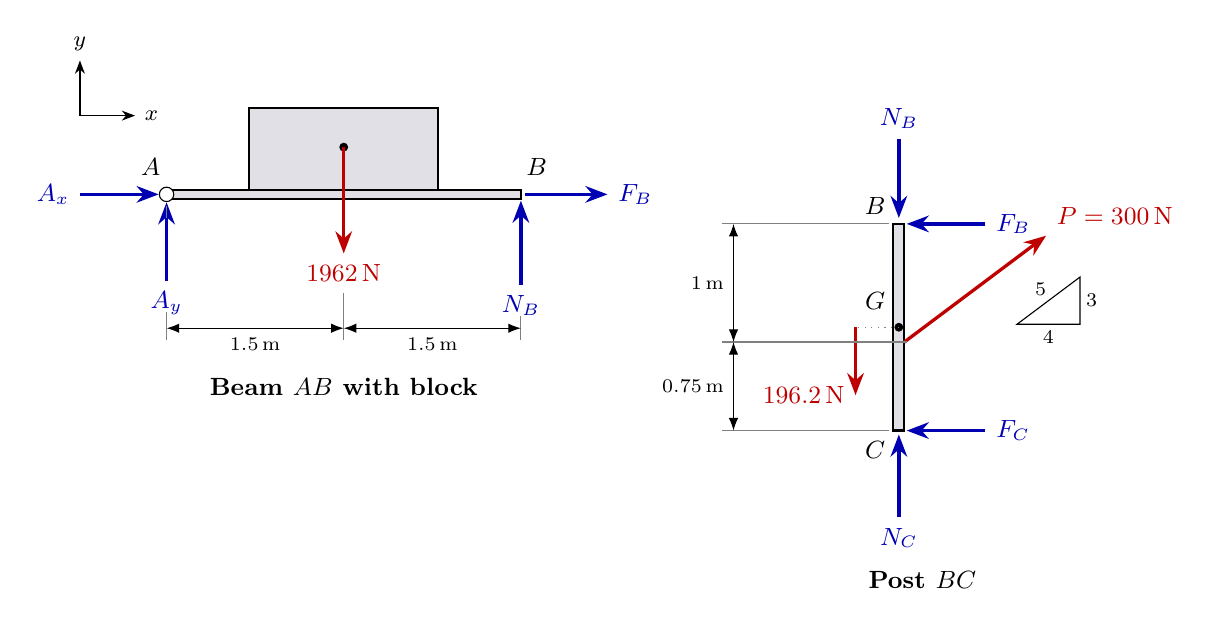
\begin{tikzpicture}[scale=1.0]
    % ---------- Beam AB + block FBD ----------
    \begin{scope}
        \draw[body] (0,-0.06) rectangle (4.5,0.06);
        \draw[body] (1.05,0.06) rectangle (3.45,1.1);
        \fill[white] (0,0) circle (2.6pt); \draw (0,0) circle (2.6pt);
        \node[lbl] at (-0.2,0.35) {$A$};
        \node[lbl] at (4.7,0.35) {$B$};
        \fill (2.25,0.6) circle (1.6pt);
        \draw[load] (2.25,0.6) -- (2.25,-0.75) node[below, lbl]{\SI{1962}{N}};
        \draw[react] (-1.1,0) -- (-0.1,0) node[pos=0, left, lbl]{$A_x$};
        \draw[react] (0,-1.1) -- (0,-0.1) node[pos=0, below, lbl]{$A_y$};
        \draw[react] (4.5,-1.15) -- (4.5,-0.08) node[pos=0, below, lbl]{$N_B$};
        \draw[react] (4.55,0) -- (5.6,0) node[right, lbl]{$F_B$};
        \draw[ext] (0,-0.15) -- (0,-0.3);
        \draw[ext] (2.25,-1.25) -- (2.25,-1.85);
        \draw[ext] (0,-1.5) -- (0,-1.85);
        \draw[ext] (4.5,-1.55) -- (4.5,-1.85);
        \draw[dim] (0,-1.7) -- (2.25,-1.7) node[midway, below, font=\scriptsize]{\SI{1.5}{m}};
        \draw[dim] (2.25,-1.7) -- (4.5,-1.7) node[midway, below, font=\scriptsize]{\SI{1.5}{m}};
        \node[font=\bfseries\small] at (2.25,-2.45) {Beam $AB$ with block};
        \axes{(-1.1,1.0)}
    \end{scope}

    % ---------- Post BC FBD ----------
    \begin{scope}[shift={(9.3,-3.0)}]
        \draw[body] (-0.07,0) rectangle (0.07,2.625);
        \node[lbl] at (-0.3,2.85) {$B$};
        \node[lbl] at (-0.3,-0.25) {$C$};
        \draw[react] (0,3.7) -- (0,2.7) node[pos=0, above, lbl]{$N_B$};
        \draw[react] (1.1,2.625) -- (0.1,2.625) node[pos=0, right, lbl]{$F_B$};
        \draw[react] (0,-1.1) -- (0,-0.05) node[pos=0, below, lbl]{$N_C$};
        \draw[react] (1.1,0) -- (0.1,0) node[pos=0, right, lbl]{$F_C$};
        \fill (0,1.3125) circle (1.6pt); \node[lbl] at (-0.3,1.65) {$G$};
        \draw[ext, dotted] (0,1.3125) -- (-0.55,1.3125);
        \draw[load] (-0.55,1.3125) -- (-0.55,0.45) node[left, lbl]{\SI{196.2}{N}};
        % P
        \draw[load] (0.07,1.125) -- ++(1.8,1.35) node[above right, lbl]{$P = \SI{300}{N}$};
        \draw[thin] (1.5,1.35) -- (2.3,1.35) -- (2.3,1.95) -- cycle;
        \node[font=\scriptsize] at (1.9,1.18) {4};
        \node[font=\scriptsize] at (2.45,1.65) {3};
        \node[font=\scriptsize] at (1.8,1.8) {5};
        % dims
        \draw[ext] (-0.12,0) -- (-2.25,0);
        \draw[ext] (0.1,1.125) -- (-2.25,1.125);
        \draw[ext] (-0.12,2.625) -- (-2.25,2.625);
        \draw[dim] (-2.1,0) -- (-2.1,1.125) node[midway, left, font=\scriptsize]{\SI{0.75}{m}};
        \draw[dim] (-2.1,1.125) -- (-2.1,2.625) node[midway, left, font=\scriptsize]{\SI{1}{m}};
        \node[font=\bfseries\small] at (0.3,-1.9) {Post $BC$};
    \end{scope}
\end{tikzpicture}
\end{center}

$P$ pulls the post to the right, so at impending slip the friction on the post at both $B$ and $C$ points left. The reaction pair at $B$ acts on the beam in the opposite directions. The post has negligible thickness, so all vertical forces on it pass through $C$.

\textbf{Solution:}

\textit{Loads.} $W_{\text{block}} = (\SI{200}{kg})(\SI{9.81}{m/s^2}) = \SI{1962}{N}$, $W_{\text{post}} = (\SI{20}{kg})(\SI{9.81}{m/s^2}) = \SI{196.2}{N}$
\[
    P_x = \tfrac{4}{5}(\SI{300}{N}) = \SI{240}{N}, \qquad P_y = \tfrac{3}{5}(\SI{300}{N}) = \SI{180}{N}
\]

\textit{Beam $AB$.} Moments about $A$ give the normal force the post must carry:
\begin{align*}
    \sum M_A &= N_B(\SI{3}{m}) - (\SI{1962}{N})(\SI{1.5}{m}) = 0 &&\Rightarrow\quad N_B = \SI{981}{N}
\end{align*}

\textit{Post $BC$.} Both ends slip, so the post translates without rotating, and moment equilibrium about $C$ splits $P_x$ between the two friction forces:
\begin{align*}
    \sum M_C &= F_B(\SI{1.75}{m}) - (\SI{240}{N})(\SI{0.75}{m}) = 0 &&\Rightarrow\quad F_B = \SI{102.9}{N} \\
    \sum F_x &= \SI{240}{N} - F_B - F_C = 0 &&\Rightarrow\quad F_C = \SI{137.1}{N} \\
    \sum F_y &= N_C - N_B - \SI{196.2}{N} + \SI{180}{N} = 0 &&\Rightarrow\quad N_C = \SI{997.2}{N}
\end{align*}

\textit{Coefficients for simultaneous slip.} Set $F = \mu_s N$ at both contacts:
\[
    \mu_B = \frac{F_B}{N_B} = \frac{\SI{102.9}{N}}{\SI{981}{N}} = 0.105, \qquad
    \mu_C = \frac{F_C}{N_C} = \frac{\SI{137.1}{N}}{\SI{997.2}{N}} = 0.138
\]

\begin{finalanswer}
    $\mu_B = 0.105$, \qquad $\mu_C = 0.138$
\end{finalanswer}

% =========================================================
% PROBLEM 6
% =========================================================
\problem{6}

\textbf{Given / Find:} Two weightless blocks. A spring ($k = \SI{20}{\lb/\inch}$, compressed \SI{5}{\inch}) presses block $A$ down; $A$'s right face rides a vertical wall and its lower face is inclined $60^\circ$ from that wall ($30^\circ$ from horizontal), resting on $B$. Block $B$ rests on a fixed $45^\circ$ slope. A smooth-tipped screw pushes horizontally on $B$ with force $P$. $\mu_s = 0.3$ at every other contact. Find the smallest $P$ that starts $B$ moving down the slope.

\textbf{Sketch:}

\begin{center}
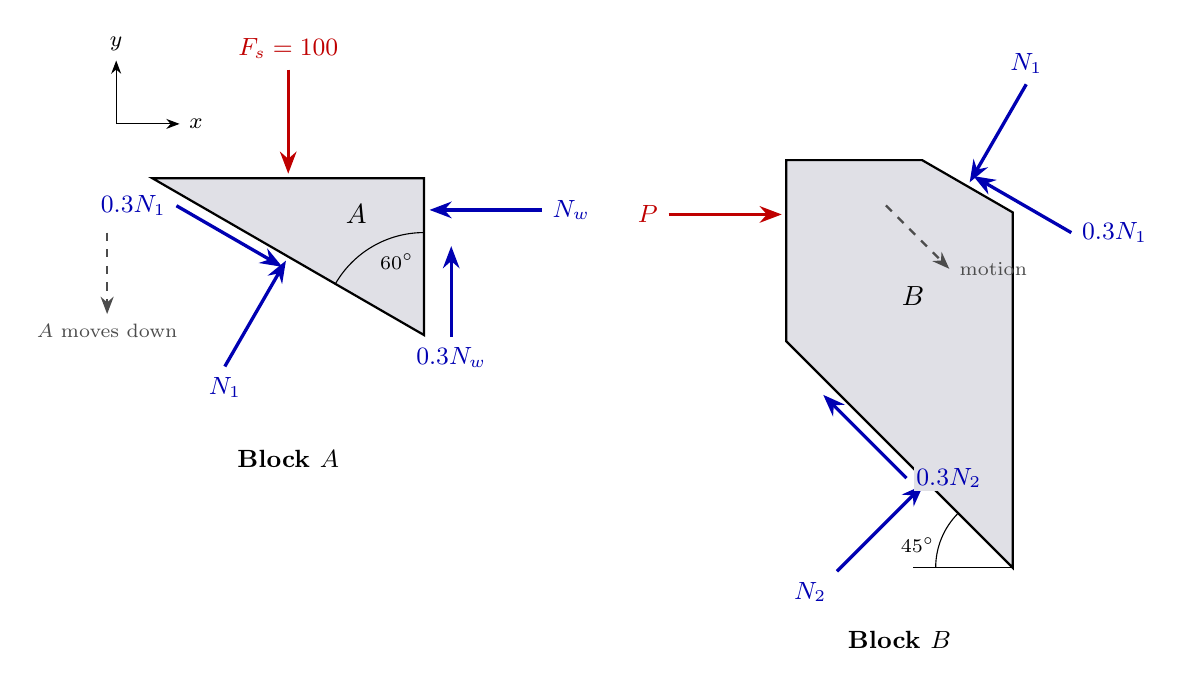
\begin{tikzpicture}[scale=1.15]
    % ---------- Block A ----------
    \begin{scope}
        \coordinate (TL) at (-3,0); \coordinate (TR) at (0,0); \coordinate (BR) at (0,-1.732);
        \coordinate (M) at (-1.5,-0.866);
        \draw[body] (TL) -- (TR) -- (BR) -- cycle;
        \node[font=\bfseries] at (-0.75,-0.4) {$A$};
        \draw[thin] (0,-0.6) arc[start angle=90, end angle=150, radius=1.13];
        \node[font=\scriptsize] at (-0.3,-0.92) {$60^\circ$};
        \draw[load] (-1.5,1.2) -- (-1.5,0.05) node[pos=0, above, lbl]{$F_s = \SI{100}{\lb}$};
        \draw[react] (1.3,-0.35) -- (0.06,-0.35) node[pos=0, right, lbl]{$N_w$};
        \draw[react] (0.3,-1.75) -- (0.3,-0.75) node[pos=0, below, lbl]{$0.3N_w$};
        \draw[react] ($(M)+(240:1.4)$) -- ($(M)+(240:0.05)$) node[pos=0, below, lbl]{$N_1$};
        \draw[react] ($(M)+(150:1.35)+(240:0.13)$) -- ($(M)+(240:0.13)$) node[pos=0, left, lbl]{$0.3N_1$};
        \draw[motion] (-3.5,-0.6) -- (-3.5,-1.5) node[below, font=\scriptsize]{$A$ moves down};
        \node[font=\bfseries\small] at (-1.5,-3.1) {Block $A$};
        \axes{(-3.4,0.6)}
    \end{scope}

    % ---------- Block B ----------
    \begin{scope}[shift={(4.0,0.2)}]
        \coordinate (P1) at (0,0); \coordinate (P2) at (1.5,0); \coordinate (P3) at (2.5,-0.577);
        \coordinate (P4) at (2.5,-4.5); \coordinate (P5) at (0,-2.0);
        \coordinate (M) at (2.0,-0.2887); \coordinate (M3) at (1.55,-3.55); \coordinate (Q) at (0.5,-2.5);
        \draw[body] (P1) -- (P2) -- (P3) -- (P4) -- (P5) -- cycle;
        \node[font=\bfseries] at (1.4,-1.5) {$B$};
        \draw[load] (-1.3,-0.6) -- (-0.05,-0.6) node[pos=0, left, lbl]{$P$};
        % from A
        \draw[react] ($(M)+(60:1.3)$) -- ($(M)+(60:0.05)$) node[pos=0, above, lbl]{$N_1$};
        \draw[react] ($(M)+(-30:1.25)+(60:0.13)$) -- ($(M)+(60:0.13)$) node[pos=0, right, lbl]{$0.3N_1$};
        % from slope
        \draw[react] ($(M3)+(225:1.4)$) -- ($(M3)+(225:0.05)$) node[pos=0, below left, lbl]{$N_2$};
        \draw[react] ($(Q)+(-45:1.3)+(225:0.13)$) -- ($(Q)+(225:0.13)$) node[pos=0, right, lbl, fill=blue!10!gray!22, inner sep=1pt, xshift=2pt]{$0.3N_2$};
        \draw[thin] (2.5,-4.5) -- (1.4,-4.5);
        \draw[thin] (1.65,-4.5) arc[start angle=180, end angle=135, radius=0.85];
        \node[font=\scriptsize] at (1.45,-4.25) {$45^\circ$};
        \draw[motion] (1.1,-0.5) -- (1.8,-1.2) node[right, font=\scriptsize]{motion};
        \node[font=\bfseries\small] at (1.25,-5.3) {Block $B$};
    \end{scope}
\end{tikzpicture}
\end{center}

\textit{Directions of friction.} $B$ moves down the $45^\circ$ slope by $u$ in each direction. The face between $A$ and $B$ drops only $u\tan 30^\circ = 0.577u$ over that horizontal travel, so the spring pushes $A$ down to stay in contact, and $A$ slides up and to the left relative to $B$. Friction on $A$ therefore points down-right along the $30^\circ$ face and up the wall; friction on $B$ points up-left along both of its inclined faces. The screw tip is smooth, so it applies only $P$.

\textbf{Solution:}

\textit{Spring force.} $F_s = kx = (\SI{20}{\lb/\inch})(\SI{5}{\inch}) = \SI{100}{\lb}$

\textit{Block $A$.}
\begin{align*}
    \sum F_x &= -N_w + N_1\sin 30^\circ + 0.3N_1\cos 30^\circ = 0 &&\Rightarrow\quad N_w = 0.760N_1 \\
    \sum F_y &= -\SI{100}{\lb} + 0.3N_w + N_1\cos 30^\circ - 0.3N_1\sin 30^\circ = 0
\end{align*}
Substituting $N_w$:
\[
    (0.228 + 0.716)N_1 = \SI{100}{\lb} \quad\Rightarrow\quad N_1 = \SI{105.9}{\lb}, \quad N_w = \SI{80.5}{\lb}
\]

\textit{Block $B$.}
\begin{align*}
    \sum F_y &= -N_1\cos 30^\circ + 0.3N_1\sin 30^\circ + N_2\cos 45^\circ + 0.3N_2\sin 45^\circ = 0 \\
    &\Rightarrow\quad N_2 = \frac{(0.716)(\SI{105.9}{\lb})}{0.919} = \SI{82.5}{\lb} \\[4pt]
    \sum F_x &= P - N_1\sin 30^\circ - 0.3N_1\cos 30^\circ + N_2\sin 45^\circ - 0.3N_2\cos 45^\circ = 0 \\
    &\Rightarrow\quad P = (0.760)(\SI{105.9}{\lb}) - (0.495)(\SI{82.5}{\lb}) = \SI{80.5}{\lb} - \SI{40.8}{\lb} = \SI{39.6}{\lb}
\end{align*}
Carrying full precision gives \SI{39.6}{\lb}. The posted \SI{39.7}{\lb} comes from rounding $N_1$ to \SI{106}{\lb} before the last step.

\begin{finalanswer}
    $P = \SI{39.6}{\lb}$ \quad (posted: \SI{39.7}{\lb}; difference is intermediate rounding)
\end{finalanswer}

% =========================================================
% PROBLEM 7
% =========================================================
\problem{7}

\textbf{Given / Find:} Wedge $A$ is pushed right by $P$ along floor $C$ and lifts block $B$, which carries \SI{3000}{\lb} and is guided by wall $D$. The $A$--$B$ interface is inclined $15^\circ$. $\mu_s = 0.3$ at $A$--$C$ and $B$--$D$; $\mu_s = 0.4$ at $A$--$B$. Wedge weights are neglected. Find the smallest $P$ that lifts the load.

\textbf{Sketch:}

\begin{center}
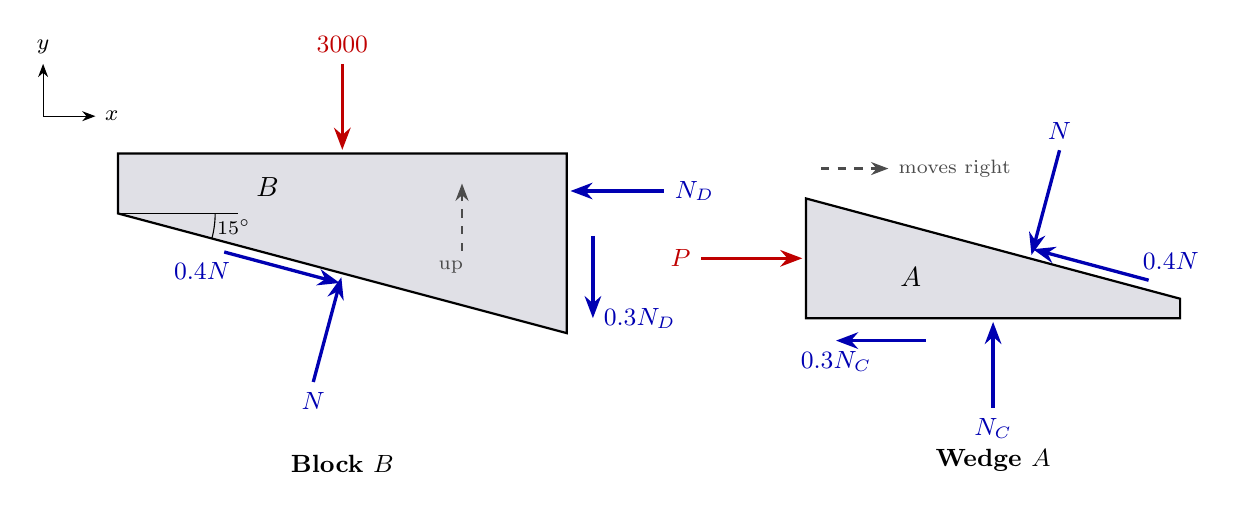
\begin{tikzpicture}[scale=0.95]
    % ---------- Block B ----------
    \begin{scope}
        \coordinate (M) at (3,0.796);
        \draw[body] (0,1.6) -- (6,0.0) -- (6,2.4) -- (0,2.4) -- cycle;
        \node[font=\bfseries] at (2.0,1.95) {$B$};
        \draw[load] (3,3.6) -- (3,2.45) node[pos=0, above, lbl]{\SI{3000}{\lb}};
        \draw[react] (7.3,1.9) -- (6.05,1.9) node[pos=0, right, lbl]{$N_D$};
        \draw[react] (6.35,1.3) -- (6.35,0.2) node[pos=1, right, lbl]{$0.3N_D$};
        \draw[react] ($(M)+(255:1.5)$) -- ($(M)+(255:0.05)$) node[pos=0, below, lbl]{$N$};
        \draw[react] ($(M)+(165:1.6)+(255:0.13)$) -- ($(M)+(255:0.13)$) node[pos=0, below left, lbl, xshift=6pt]{$0.4N$};
        \draw[thin] (0,1.6) -- (1.6,1.6);
        \draw[thin] (1.3,1.6) arc[start angle=0, end angle=-15, radius=1.3];
        \node[font=\scriptsize] at (1.55,1.42) {$15^\circ$};
        \draw[motion] (4.6,1.1) -- (4.6,2.0) node[pos=0, below, font=\scriptsize, xshift=-4pt]{up};
        \node[font=\bfseries\small] at (3,-1.75) {Block $B$};
        \axes{(-1.0,2.9)}
    \end{scope}

    % ---------- Wedge A ----------
    \begin{scope}[shift={(9.2,0.2)}]
        \coordinate (M) at (3,0.796);
        \draw[body] (0,0) -- (5,0) -- (5,0.26) -- (0,1.6) -- cycle;
        \node[font=\bfseries] at (1.4,0.55) {$A$};
        \draw[load] (-1.4,0.8) -- (-0.05,0.8) node[pos=0, left, lbl]{$P$};
        \draw[react] ($(M)+(75:1.5)$) -- ($(M)+(75:0.05)$) node[pos=0, above, lbl]{$N$};
        \draw[react] ($(M)+(-15:1.6)+(75:0.13)$) -- ($(M)+(75:0.13)$) node[pos=0, above right, lbl, xshift=-6pt]{$0.4N$};
        \draw[react] (2.5,-1.2) -- (2.5,-0.05) node[pos=0, below, lbl]{$N_C$};
        \draw[react] (1.6,-0.3) -- (0.4,-0.3) node[pos=1, below, lbl]{$0.3N_C$};
        \draw[motion] (0.2,2.0) -- (1.1,2.0) node[right, font=\scriptsize]{moves right};
        \node[font=\bfseries\small] at (2.5,-1.9) {Wedge $A$};
    \end{scope}
\end{tikzpicture}
\end{center}

As $A$ moves right, $B$ rises against the wall, so friction from $D$ on $B$ points down. Relative to $A$, block $B$ slides up and to the left along the $15^\circ$ face, so friction on $B$ points down-right along that face and friction on $A$ points up-left. Friction from the floor on $A$ points left.

\textbf{Solution:}

\textit{Block $B$.}
\begin{align*}
    \sum F_x &= N\sin 15^\circ + 0.4N\cos 15^\circ - N_D = 0 \\
    \sum F_y &= N\cos 15^\circ - 0.4N\sin 15^\circ - 0.3N_D - \SI{3000}{\lb} = 0
\end{align*}
From the first equation, $N_D = (0.259 + 0.386)N = 0.645N$. Substituting into the second:
\[
    (0.966 - 0.104 - 0.194)N = \SI{3000}{\lb} \quad\Rightarrow\quad N = \SI{4485}{\lb}, \quad N_D = \SI{2894}{\lb}
\]

\textit{Wedge $A$.}
\begin{align*}
    \sum F_y &= N_C - N\cos 15^\circ + 0.4N\sin 15^\circ = 0 &&\Rightarrow\quad N_C = \SI{3868}{\lb} \\
    \sum F_x &= P - N\sin 15^\circ - 0.4N\cos 15^\circ - 0.3N_C = 0
\end{align*}
\[
    P = \SI{1161}{\lb} + \SI{1733}{\lb} + \SI{1160}{\lb} = \SI{4054}{\lb}
\]

\begin{finalanswer}
    $P = \SI{4.05}{\kip}$ \quad (\SI{4050}{\lb})
\end{finalanswer}

% =========================================================
% PROBLEM 8
% =========================================================
\problem{8}

\textbf{Given / Find:} A \SI{50}{\lb} block on a $45^\circ$ incline ($\mu_s = 0.2$) is tied to a rope that runs parallel to the incline, over fixed drum $D$ ($\mu_s = 0.3$), and down to a hanging weight $W$. Find the minimum and maximum $W$ that keep the block from slipping.

\textbf{Sketch:}

\begin{center}
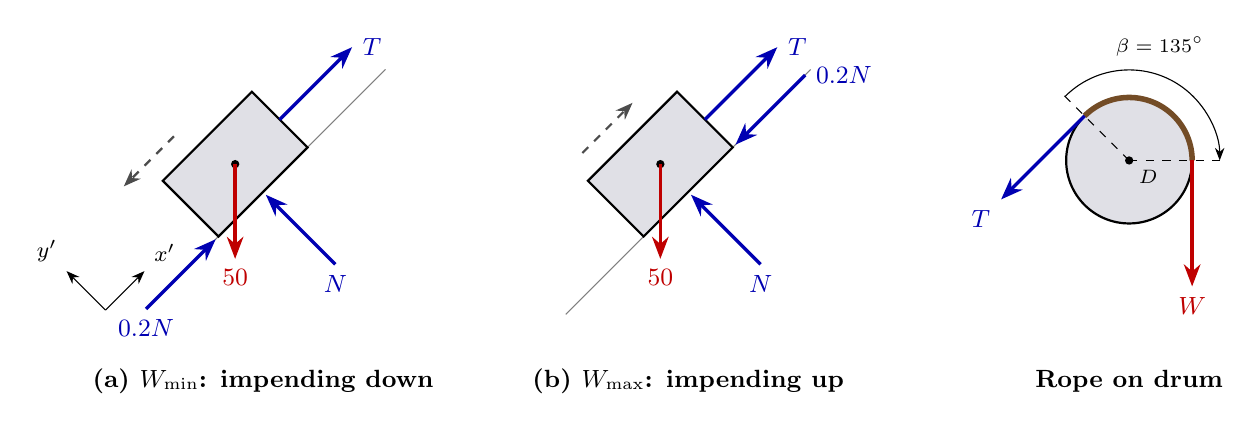
\begin{tikzpicture}[scale=1.0]
    % ---------- (a) block, impending down ----------
    \begin{scope}
        \begin{scope}[rotate=45]
            \draw[thin, gray] (-1.6,0) -- (2.2,0);
            \draw[body] (-0.8,0) rectangle (0.8,1.0);
            \fill (0,0.5) circle (1.5pt);
            \draw[react] (0.8,0.5) -- (2.1,0.5) node[right, lbl]{$T$};
            \draw[react] (0,-1.3) -- (0,-0.05) node[pos=0, below, lbl]{$N$};
            \draw[react] (-2.1,0) -- (-0.85,0) node[pos=0, below, lbl]{$0.2N$};
            \draw[motion] (-0.3,1.3) -- (-1.2,1.3);
        \end{scope}
        \draw[load] (-0.354,0.354) -- (-0.354,-0.85) node[below, lbl]{\SI{50}{\lb}};
        \node[font=\bfseries\small] at (0,-2.4) {(a) $W_{\min}$: impending down};
        \draw[-{Stealth},thin] (-2.0,-1.5) -- ++(45:0.7) node[above right, font=\footnotesize]{$x'$};
        \draw[-{Stealth},thin] (-2.0,-1.5) -- ++(135:0.7) node[above left, font=\footnotesize]{$y'$};
    \end{scope}

    % ---------- (b) block, impending up ----------
    \begin{scope}[shift={(5.4,0)}]
        \begin{scope}[rotate=45]
            \draw[thin, gray] (-2.2,0) -- (2.2,0);
            \draw[body] (-0.8,0) rectangle (0.8,1.0);
            \fill (0,0.5) circle (1.5pt);
            \draw[react] (0.8,0.5) -- (2.1,0.5) node[right, lbl]{$T$};
            \draw[react] (0,-1.3) -- (0,-0.05) node[pos=0, below, lbl]{$N$};
            \draw[react] (2.1,0) -- (0.85,0) node[pos=0, right, lbl]{$0.2N$};
            \draw[motion] (-0.6,1.3) -- (0.3,1.3);
        \end{scope}
        \draw[load] (-0.354,0.354) -- (-0.354,-0.85) node[below, lbl]{\SI{50}{\lb}};
        \node[font=\bfseries\small] at (0,-2.4) {(b) $W_{\max}$: impending up};
    \end{scope}

    % ---------- Drum ----------
    \begin{scope}[shift={(11.0,0.4)}]
        \draw[body] (0,0) circle (0.8);
        \fill (0,0) circle (1.5pt) node[below right, font=\scriptsize]{$D$};
        \draw[line width=2pt, brown!60!black] (135:0.8) arc[start angle=135, end angle=0, radius=0.8];
        \draw[react] (135:0.8) -- ++(225:1.5) node[below left, lbl]{$T$};
        \draw[load] (0.8,0) -- (0.8,-1.6) node[below, lbl]{$W$};
        \draw[thin, dashed] (0,0) -- (135:1.25);
        \draw[thin, dashed] (0,0) -- (0:1.25);
        \draw[-{Stealth[length=1.6mm]}, thin] (135:1.15) arc[start angle=135, end angle=0, radius=1.15];
        \node[font=\scriptsize] at (75:1.5) {$\beta = 135^\circ$};
        \node[font=\bfseries\small] at (0,-2.8) {Rope on drum};
    \end{scope}
\end{tikzpicture}
\end{center}

The rope leaves the drum parallel to the $45^\circ$ incline and comes off vertically, so it is in contact for $\beta = 45^\circ + 90^\circ = 135^\circ = 3\pi/4$ rad. The incline axes $x'$ (up the slope) and $y'$ (normal) are used for the block. The pin reaction at $D$ does not enter the belt-friction relation and is not needed.

\textbf{Solution:}

\textit{Belt friction on the drum.} The rope is about to slip toward the side with the larger tension:
\[
    \frac{T_2}{T_1} = e^{\mu_s\beta} = e^{(0.3)(3\pi/4)} = e^{0.707} = 2.028
\]

\textit{Block normal force} (same in both cases):
\[
    \sum F_{y'} = N - (\SI{50}{\lb})\cos 45^\circ = 0 \quad\Rightarrow\quad N = \SI{35.36}{\lb}, \qquad 0.2N = \SI{7.07}{\lb}
\]

\textit{(a) Minimum $W$: block about to slide down.} Friction on the block acts up the slope. The block side of the rope has the larger tension, $T = We^{\mu_s\beta}$.
\begin{align*}
    \sum F_{x'} &= T + 0.2N - (\SI{50}{\lb})\sin 45^\circ = 0 &&\Rightarrow\quad T = \SI{35.36}{\lb} - \SI{7.07}{\lb} = \SI{28.28}{\lb} \\
    W_{\min} &= \frac{T}{e^{\mu_s\beta}} = \frac{\SI{28.28}{\lb}}{2.028} = \SI{13.9}{\lb}
\end{align*}

\textit{(b) Maximum $W$: block about to slide up.} Friction on the block acts down the slope. The hanging side has the larger tension, $W = Te^{\mu_s\beta}$.
\begin{align*}
    \sum F_{x'} &= T - 0.2N - (\SI{50}{\lb})\sin 45^\circ = 0 &&\Rightarrow\quad T = \SI{35.36}{\lb} + \SI{7.07}{\lb} = \SI{42.43}{\lb} \\
    W_{\max} &= Te^{\mu_s\beta} = (\SI{42.43}{\lb})(2.028) = \SI{86.0}{\lb}
\end{align*}

\begin{finalanswer}
    $W_{\min} = \SI{13.9}{\lb}$ (below this the block slips down the slope) \\
    $W_{\max} = \SI{86.0}{\lb}$ (above this the block slides up the slope)
\end{finalanswer}

% =========================================================
% PROBLEM 9
% =========================================================
\problem{9}

\textbf{Given / Find:} Block $B$ (\SI{30}{\lb}) sits on block $A$ (\SI{50}{\lb}) along a face inclined $20^\circ$ ($\mu_{BA} = 0.6$), and $A$ rests on floor $C$ ($\mu_{AC} = 0.4$). A horizontal rope from the left side of $B$ passes \SI{90}{\degree} over a fixed peg ($\mu = 0.5$) and holds block $D$. Find the largest weight $W_D$ that does not cause motion.

\textbf{Sketch:}

\begin{center}
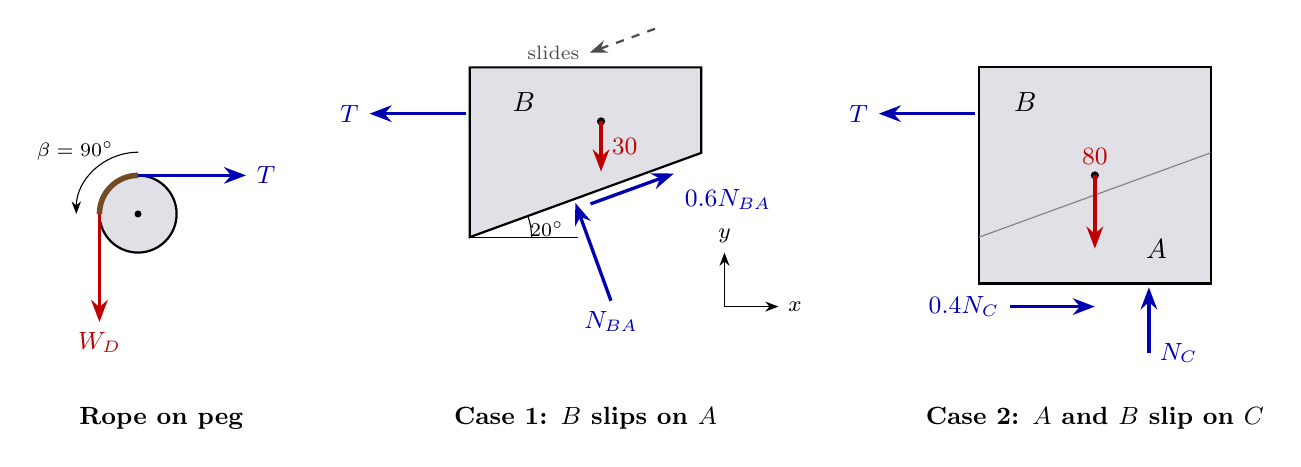
\begin{tikzpicture}[scale=0.98]
    % ---------- Peg ----------
    \begin{scope}
        \draw[body] (0,0) circle (0.5);
        \fill (0,0) circle (1.3pt);
        \draw[line width=2pt, brown!60!black] (90:0.5) arc[start angle=90, end angle=180, radius=0.5];
        \draw[react] (0,0.5) -- (1.4,0.5) node[right, lbl]{$T$};
        \draw[load] (-0.5,0) -- (-0.5,-1.4) node[below, lbl]{$W_D$};
        \draw[-{Stealth[length=1.6mm]}, thin] (90:0.8) arc[start angle=90, end angle=180, radius=0.8];
        \node[font=\scriptsize] at (135:1.15) {$\beta = 90^\circ$};
        \node[font=\bfseries\small] at (0.3,-2.65) {Rope on peg};
    \end{scope}

    % ---------- Case 1: block B alone ----------
    \begin{scope}[shift={(4.3,-0.9)}]
        \coordinate (M) at (1.35,1.091); \coordinate (Q) at (2.6,1.546);
        \draw[body] (0,0.6) -- (3,1.692) -- (3,2.8) -- (0,2.8) -- cycle;
        \node[font=\bfseries] at (0.7,2.35) {$B$};
        \draw[react] (-0.05,2.2) -- (-1.3,2.2) node[left, lbl]{$T$};
        \fill (1.7,2.1) circle (1.5pt);
        \draw[load] (1.7,2.1) -- (1.7,1.45) node[pos=0.5, right, lbl]{\SI{30}{\lb}};
        \draw[react] ($(M)+(290:1.4)$) -- ($(M)+(290:0.05)$) node[pos=0, below, lbl]{$N_{BA}$};
        \draw[react] ($(Q)+(200:1.15)+(290:0.13)$) -- ($(Q)+(290:0.13)$) node[pos=1, below right, lbl, yshift=-2pt]{$0.6N_{BA}$};
        \draw[thin] (0,0.6) -- (1.4,0.6);
        \draw[thin] (0.8,0.6) arc[start angle=0, end angle=20, radius=0.8];
        \node[font=\scriptsize] at (1.0,0.7) {$20^\circ$};
        \draw[motion] (2.4,3.3) -- ++(200:0.9) node[left, font=\scriptsize]{slides};
        \node[font=\bfseries\small] at (1.5,-1.75) {Case 1: $B$ slips on $A$};
        \axes{(3.3,-0.3)}
    \end{scope}

    % ---------- Case 2: A and B together ----------
    \begin{scope}[shift={(10.9,-0.9)}]
        \draw[body] (0,0) rectangle (3,2.8);
        \draw[thin, gray] (0,0.6) -- (3,1.692);
        \node[font=\bfseries] at (0.6,2.35) {$B$};
        \node[font=\bfseries] at (2.3,0.45) {$A$};
        \draw[react] (-0.05,2.2) -- (-1.3,2.2) node[left, lbl]{$T$};
        \fill (1.5,1.4) circle (1.5pt);
        \draw[load] (1.5,1.4) -- (1.5,0.45) node[pos=0, above, lbl]{\SI{80}{\lb}};
        \draw[react] (2.2,-0.9) -- (2.2,-0.05) node[pos=0, right, lbl]{$N_C$};
        \draw[react] (0.4,-0.3) -- (1.5,-0.3) node[pos=0, left, lbl]{$0.4N_C$};
        \node[font=\bfseries\small] at (1.5,-1.75) {Case 2: $A$ and $B$ slip on $C$};
    \end{scope}
\end{tikzpicture}
\end{center}

Motion can start in two ways: $B$ slides down-left along the $20^\circ$ face while $A$ stays put, or $A$ and $B$ slide left together on the floor. Both are checked, and the smaller $W_D$ governs. In either case $D$ is falling, so the rope slips toward the hanging side and $W_D$ is the larger tension.

\textbf{Solution:}

\textit{Belt friction on the peg.}
\[
    W_D = Te^{\mu\beta} = Te^{(0.5)(\pi/2)} = 2.193\,T
\]

\textit{Case 1: $B$ slips on $A$.} Friction on $B$ points up-right along the face; $N_{BA}$ is perpendicular to the face.
\begin{align*}
    \sum F_y &= N_{BA}\cos 20^\circ + 0.6N_{BA}\sin 20^\circ - \SI{30}{\lb} = 0 &&\Rightarrow\quad N_{BA} = \frac{\SI{30}{\lb}}{1.145} = \SI{26.20}{\lb} \\
    \sum F_x &= -T - N_{BA}\sin 20^\circ + 0.6N_{BA}\cos 20^\circ = 0 &&\Rightarrow\quad T = (0.222)(\SI{26.20}{\lb}) = \SI{5.81}{\lb}
\end{align*}
\[
    W_D = (2.193)(\SI{5.81}{\lb}) = \SI{12.7}{\lb}
\]
Check that $A$ stays put: the horizontal force $B$ transfers to $A$ equals $T = \SI{5.81}{\lb}$, well below the \SI{32.0}{\lb} the floor can hold (Case 2).

\textit{Case 2: $A$ and $B$ slip together on $C$.}
\begin{align*}
    \sum F_y &= N_C - \SI{80}{\lb} = 0 &&\Rightarrow\quad N_C = \SI{80.0}{\lb} \\
    \sum F_x &= -T + 0.4N_C = 0 &&\Rightarrow\quad T = \SI{32.0}{\lb}
\end{align*}
\[
    W_D = (2.193)(\SI{32.0}{\lb}) = \SI{70.2}{\lb}
\]

Case 1 requires the smaller weight, so $B$ slipping on $A$ is what starts the motion.

\begin{finalanswer}
    $W_D = \SI{12.7}{\lb}$ \\ $B$ slips on $A$ first; sliding $A$ and $B$ together would need \SI{70.2}{\lb}.
\end{finalanswer}

\end{document}